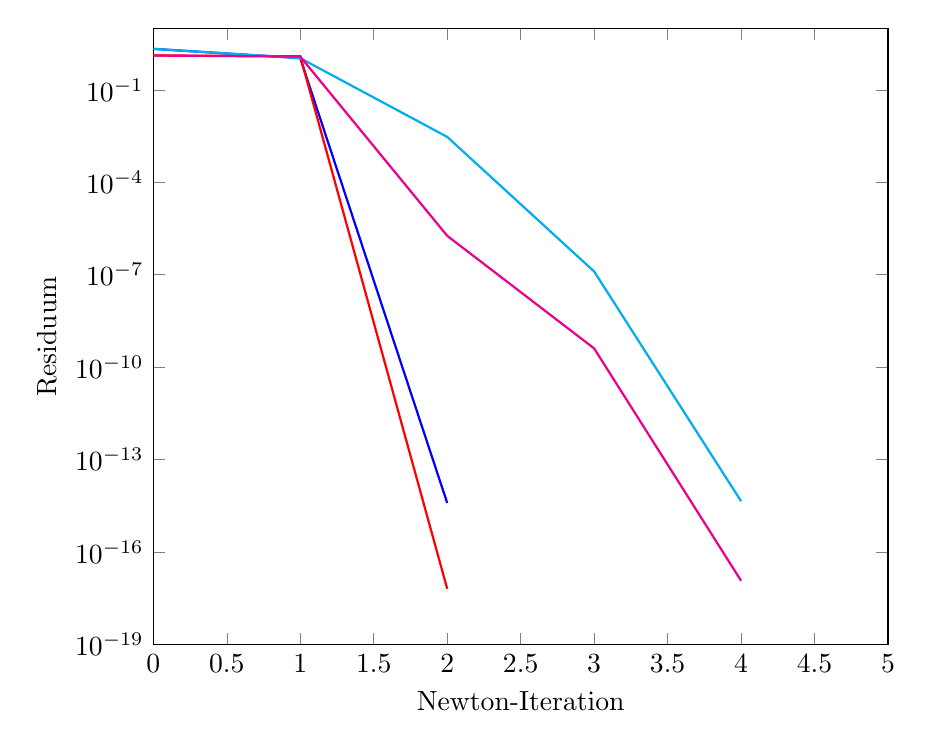
\begin{tikzpicture}[every plot/.append style={thick}] 
\begin{axis}[ 
label style={font=\normalsize}, 
xlabel={Newton-Iteration}, 
ylabel={Residuum}, 
xmin=0, xmax=5, 
ymode=log, 
ymin=0, ymax=10, 
width=0.9\textwidth, 
grid style=dashed, 
] 
\addplot[ 
color=blue, 
] 
coordinates { 
(0, 2.14e+00)(1, 1.07e+00)(2, 3.91e-15)}; 
\addplot[ 
color=red, 
] 
coordinates { 
(0, 1.31e+00)(1, 1.23e+00)(2, 6.39e-18)}; 
\addplot[ 
color=cyan, 
] 
coordinates { 
(0, 2.14e+00)(1, 1.07e+00)(2, 2.97e-03)(3, 1.27e-07)(4, 4.43e-15)}; 
\addplot[ 
color=magenta, 
] 
coordinates { 
(0, 1.30e+00)(1, 1.20e+00)(2, 1.83e-06)(3, 4.04e-10)(4, 1.16e-17)}; 
\end{axis} 
\end{tikzpicture} 
